\documentclass[a4paper]{article}
\usepackage{ctex}
\usepackage[margin=1in]{geometry}
\usepackage{listings}
\lstset{tabsize=3}
\usepackage{graphicx}
\usepackage{amsmath}
\usepackage{subfigure}
\usepackage{caption}
\usepackage{multirow}
\usepackage[backend=biber,style=authoryear,sorting=none]{biblatex}
\addbibresource{refer.bib}
\usepackage[ruled]{algorithm2e}
\usepackage{fancyhdr}
\chead{}
\rhead{W.J.Z All rights reserved}
\lhead{}
\pagestyle{fancy}
\graphicspath{{picture/}}
\title{{Latex 论文写作总结}\\
{ \large second edition} }
\author{W.J.Z}
\date{2019.4.3}
\begin{document}
	\maketitle
	\begin{abstract}
		本次是第二个版本,在第一版的基础上增加了一些更为细节和高级的排版,同时添加示例可以直接的观察到代码所要显示的效果。
	\end{abstract}
	\section{Latex}
	\subsection{a4纸设置}
	\begin{lstlisting}
	\documentclass[a4paper]{article}
	\usepackage[margin=1in]{geometry}
	\end{lstlisting}
	\subsection{中文设置}
	\begin{lstlisting}
	1、Options->Configure->bulid->Default complier->Xelatex/
	2、TeXstudio右下角设置为UTF-8.
	3、使用中文支持包 \usepackage{ctex}.
	\end{lstlisting}
	\subsection{论文结构}
	\begin{lstlisting}
	一级标题:\section{一级标题}
	二级标题:\subseciton{二级标题}
	三级标题:\subsubsection{三级标题}
	以此类推
	\end{lstlisting}
	\subsection{插图}
	\begin{lstlisting}
	1、加载支持包
		\usepackage{graphicx}
		\usepackage{subfigure}
		\usepackage{epstopdf} #eps图片支持
	2、设置图片文件夹路径
		\graphicspath{{picture/}} #当前目录下picture文件夹下
	3、单张图片
		\begin{figure}[htbp]         %h:here;t:top;b:bottom;p:page
			\centering
			\caption{图片名称}
			\includegraphics[scale=0.5][apple.eps]
			\label{apple}
		\end{figure}
	\end{lstlisting}
	\begin{figure}[htbp]
		\centering
		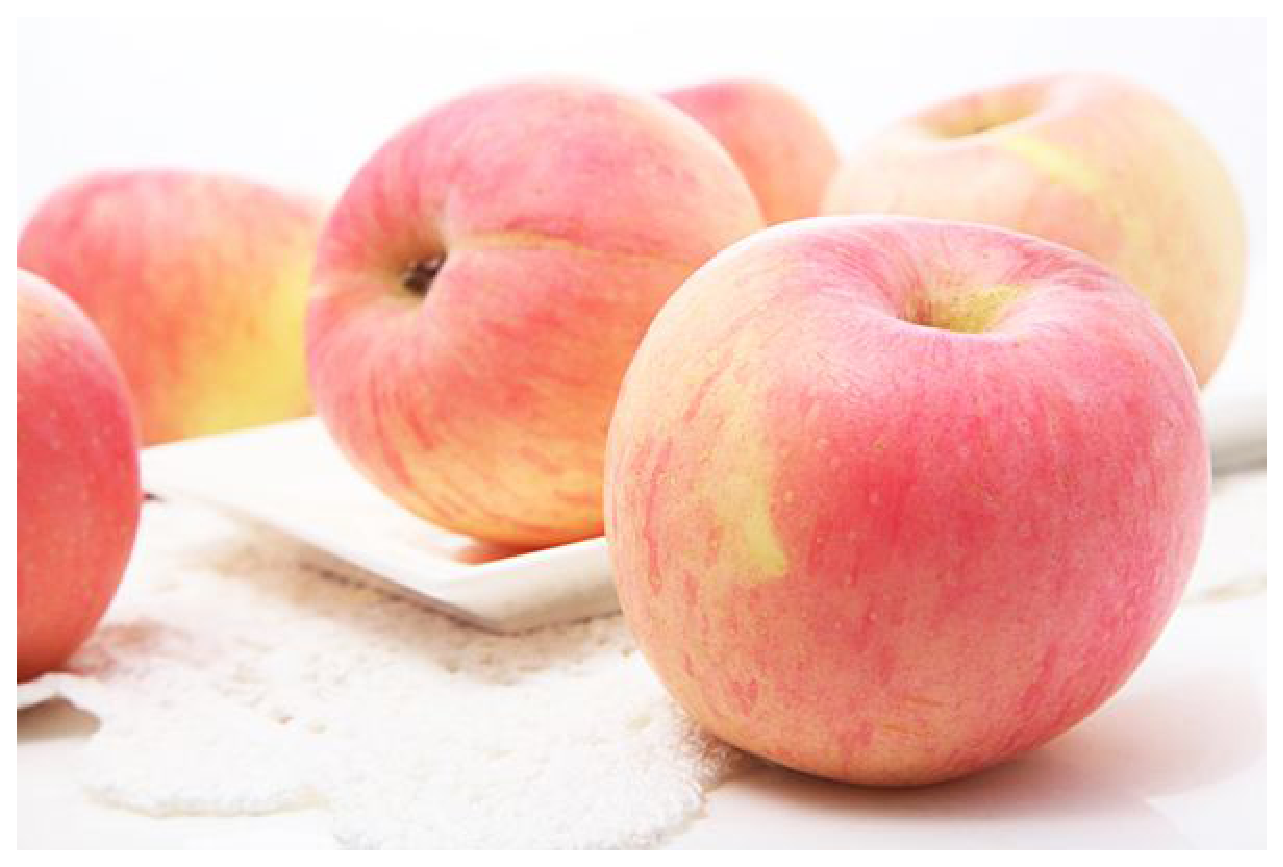
\includegraphics[scale=0.2]{apple.eps}
		\caption{apple}
	\end{figure}
	\begin{lstlisting}
	4、多张图片排版
		\begin{figure}
			\begin{minipage}[b]{0.45\textwidth}
				\centering
				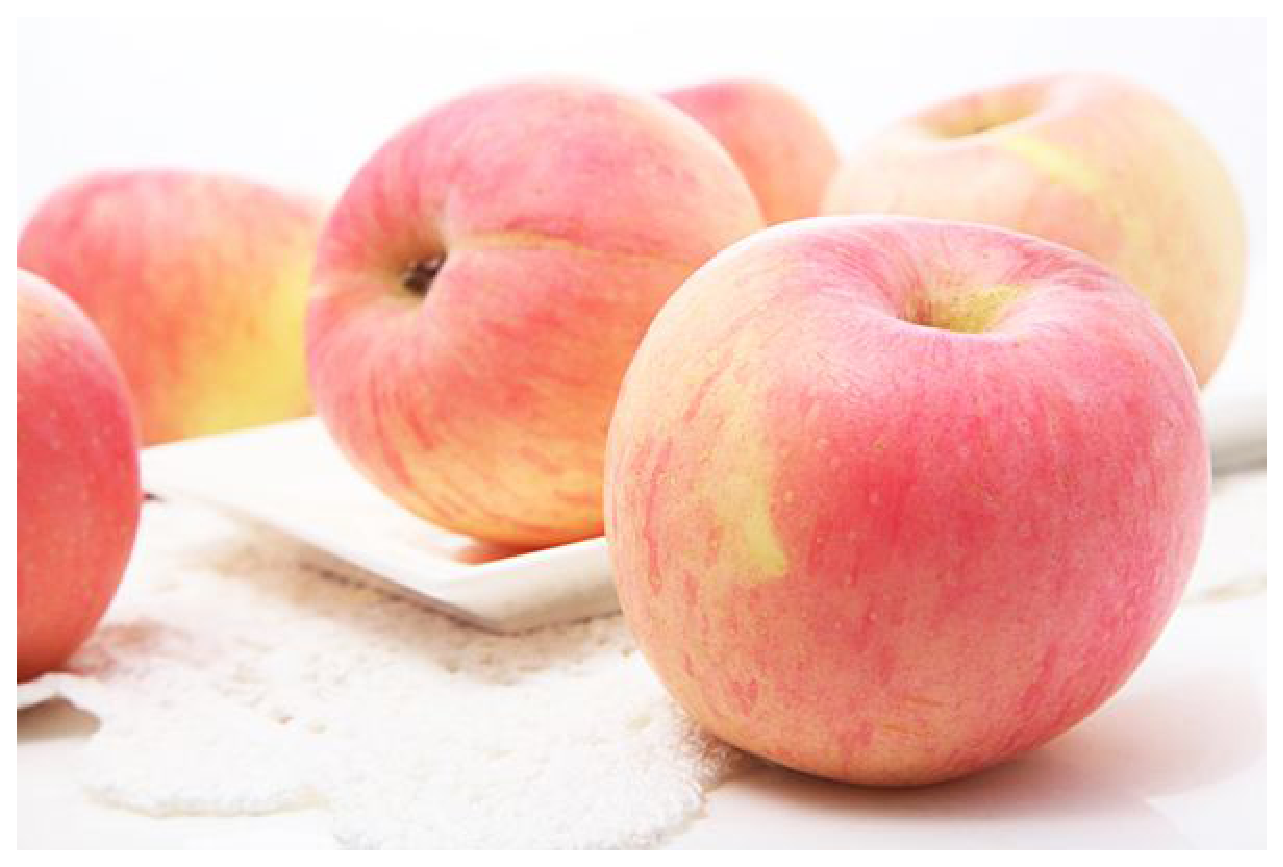
\includegraphics[scale=0.15]{apple.eps}
				\caption*{apple1}
			\end{minipage}
			\begin{minipage}[b]{0.45\textwidth}
				\centering
				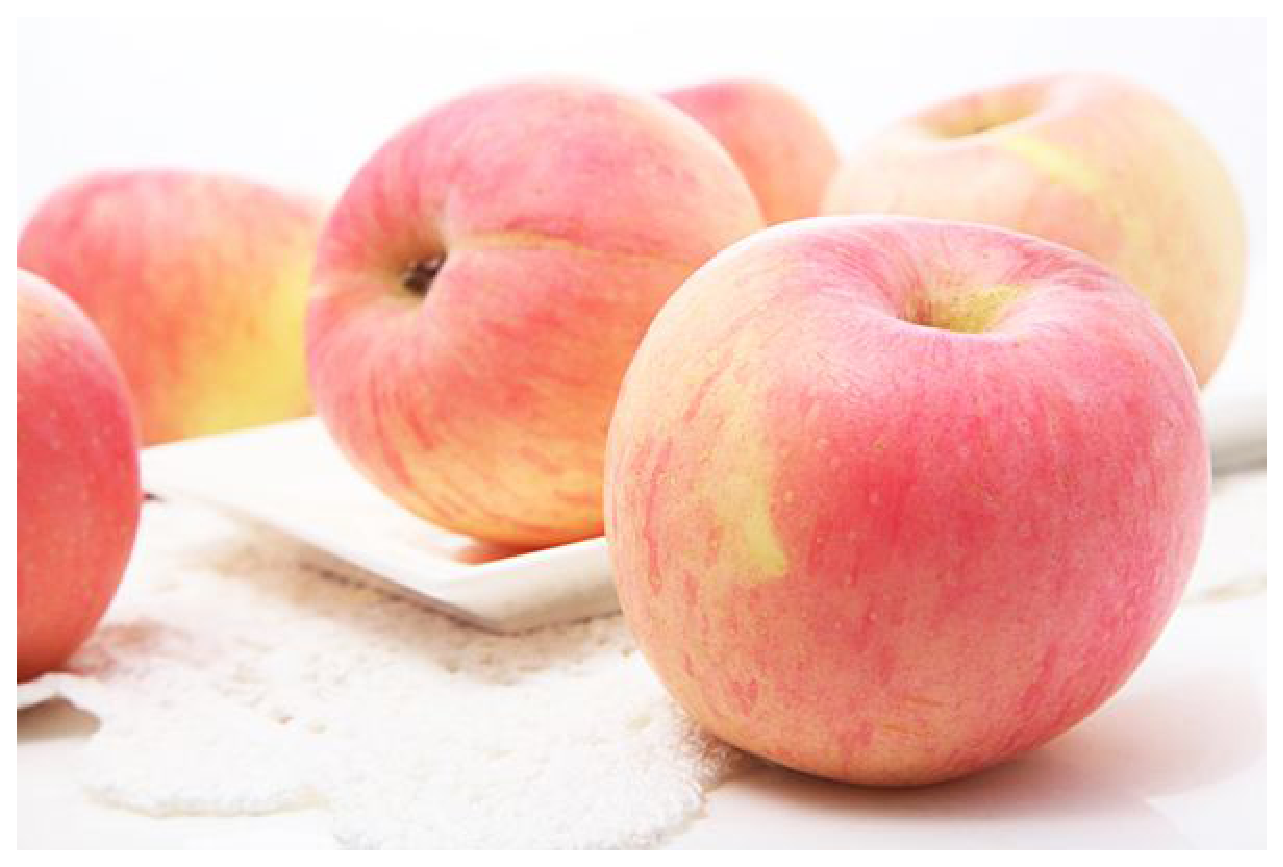
\includegraphics[scale=0.15]{apple.eps}
				\caption{apple2}
			\end{minipage}
			\begin{minipage}[b]{0.45\textwidth}
				\centering
				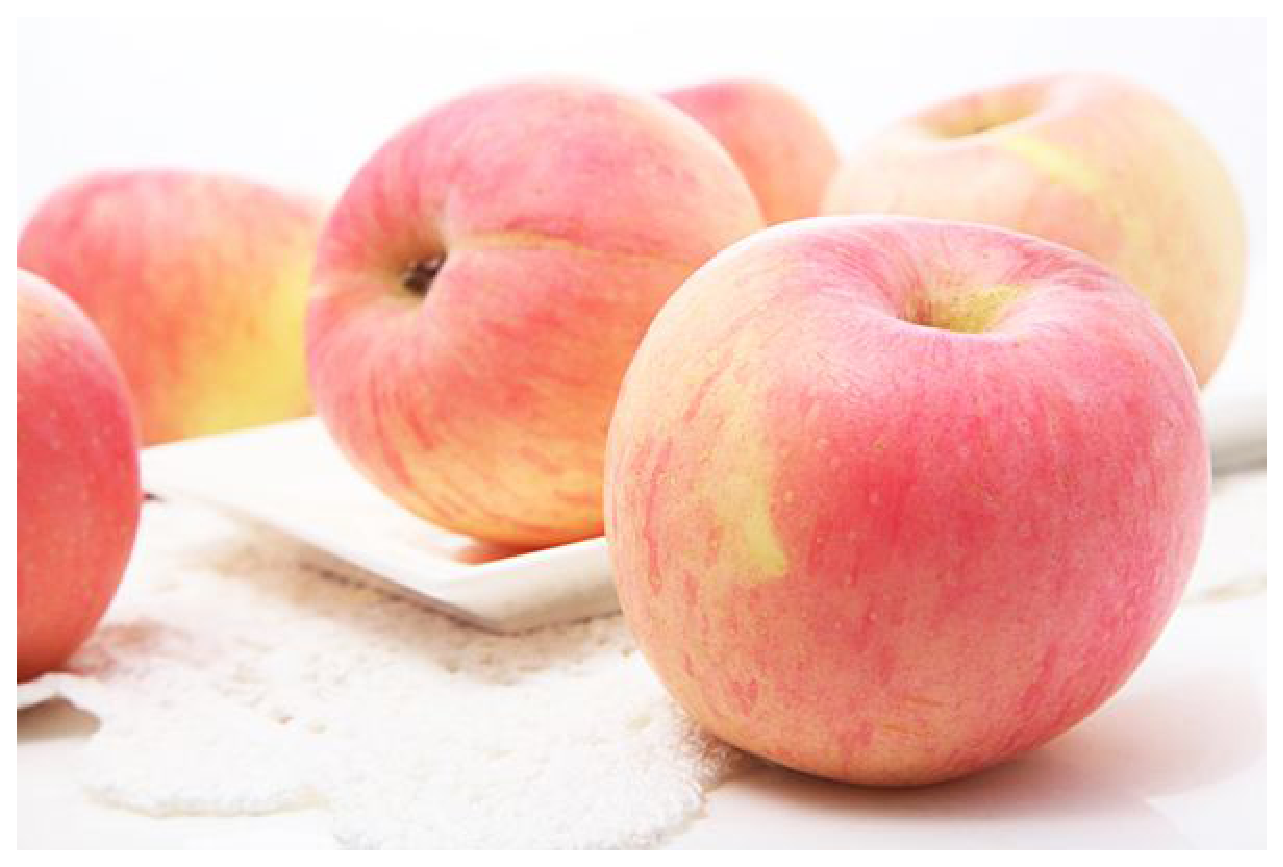
\includegraphics[scale=0.15]{apple.eps}
				\caption{apple3}
			\end{minipage}
				\begin{minipage}[b]{0.45\textwidth}
			\centering
			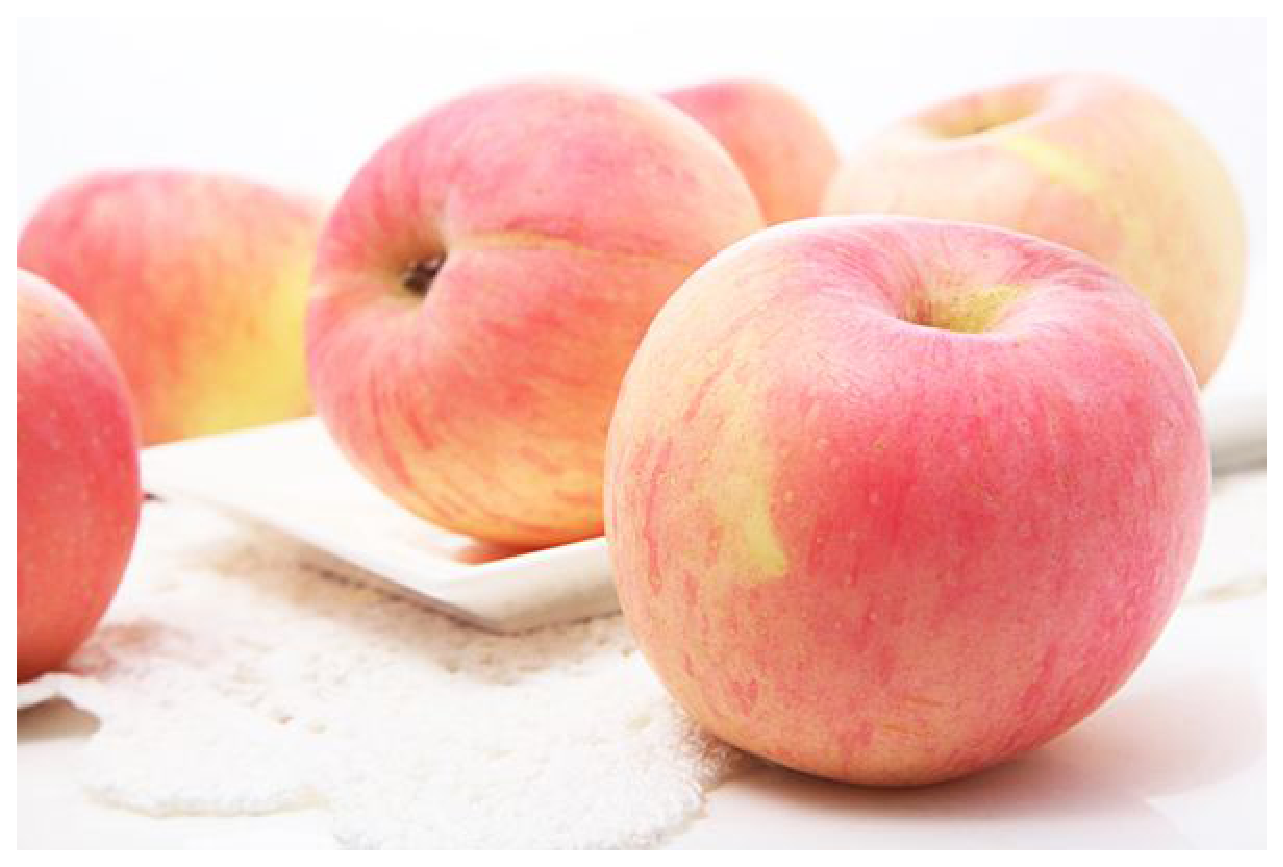
\includegraphics[scale=0.15]{apple.eps}
			\caption{apple4}
			\end{minipage}
			\caption*{apple}
		\end{figure}
	\end{lstlisting}
	\begin{figure}[htbp]
		\centering
		\begin{minipage}[b]{0.45\textwidth}
			\centering
			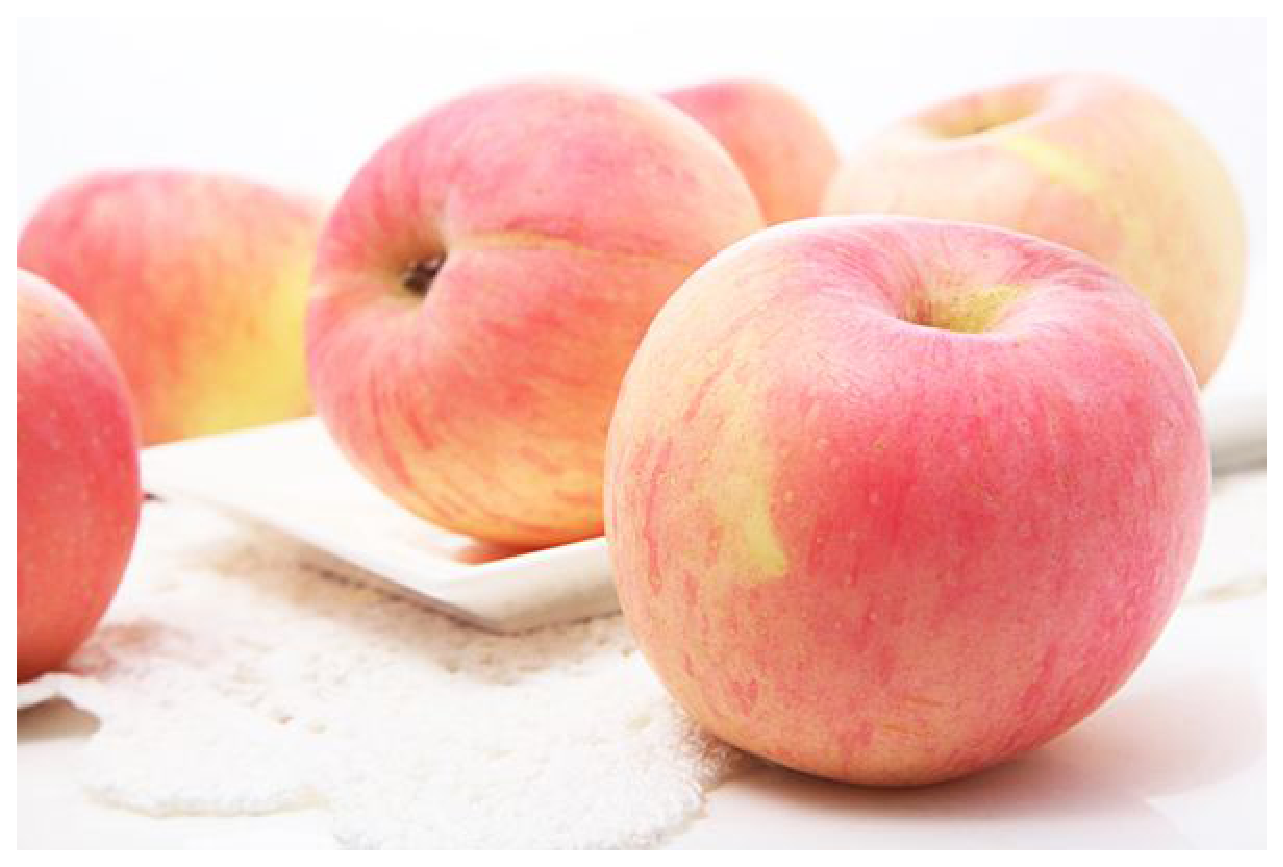
\includegraphics[scale=0.15]{apple.eps}
			\caption{apple1}
		\end{minipage}
		\begin{minipage}[b]{0.45\textwidth}
			\centering
			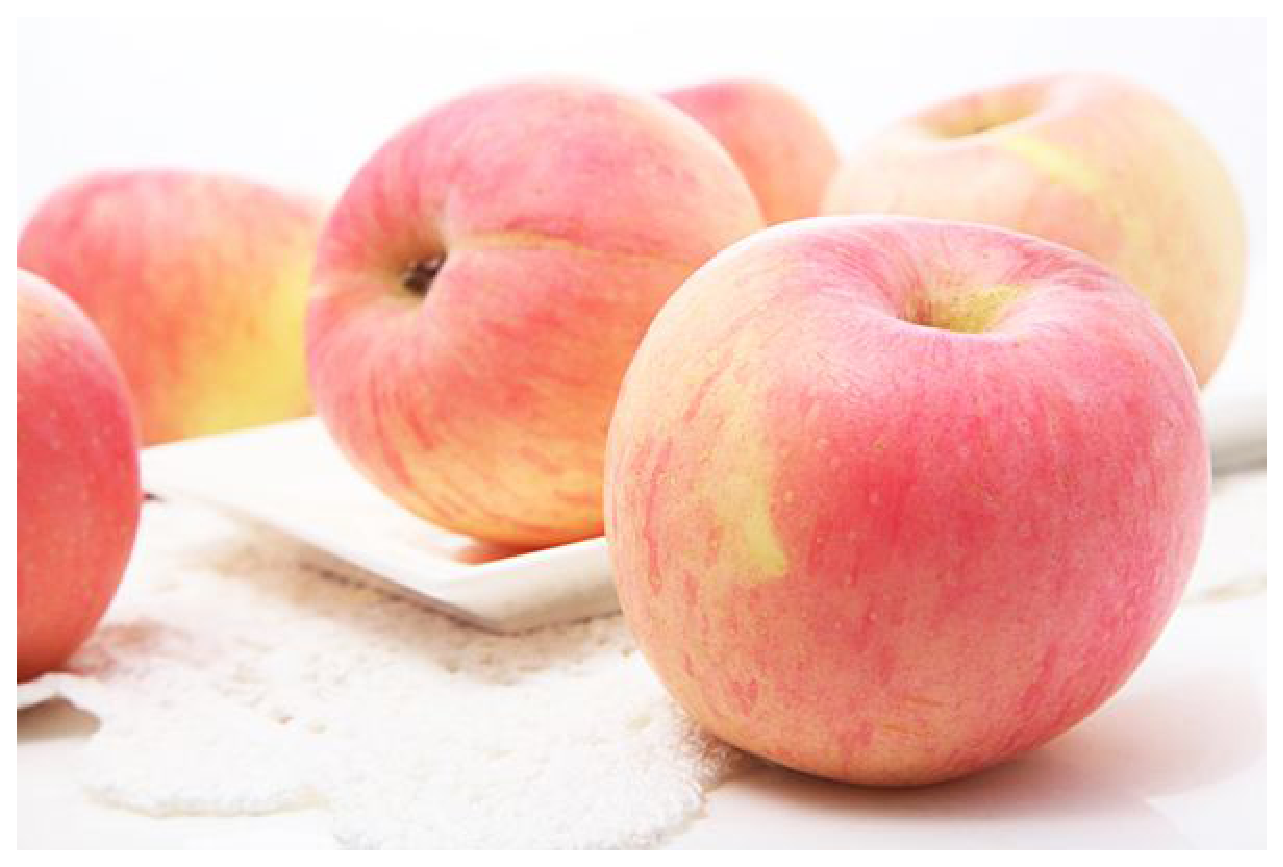
\includegraphics[scale=0.15]{apple.eps}
			\caption{apple2}
		\end{minipage}
		\begin{minipage}[b]{0.45\textwidth}
			\centering
			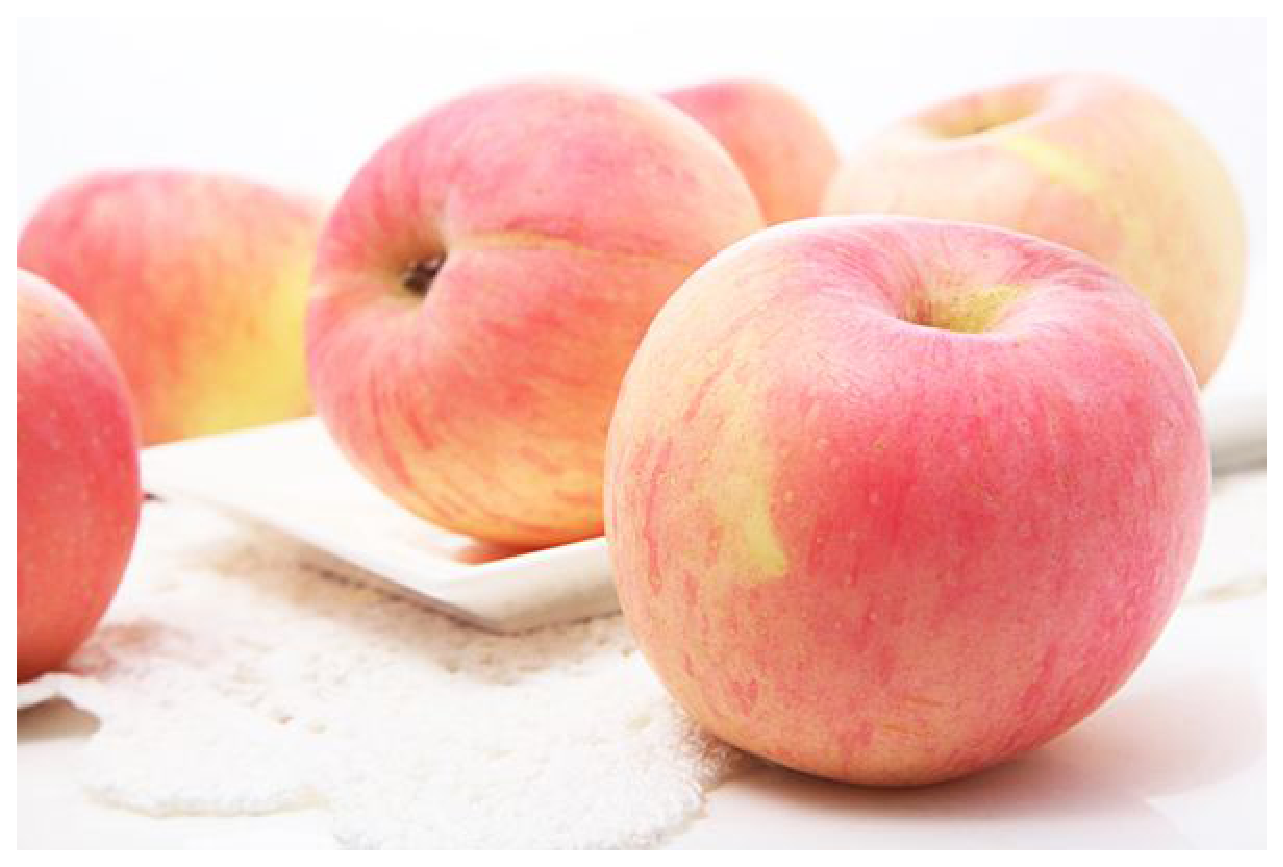
\includegraphics[scale=0.15]{apple.eps}
			\caption{apple3}
		\end{minipage}
	\begin{minipage}[b]{0.45\textwidth}
		\centering
		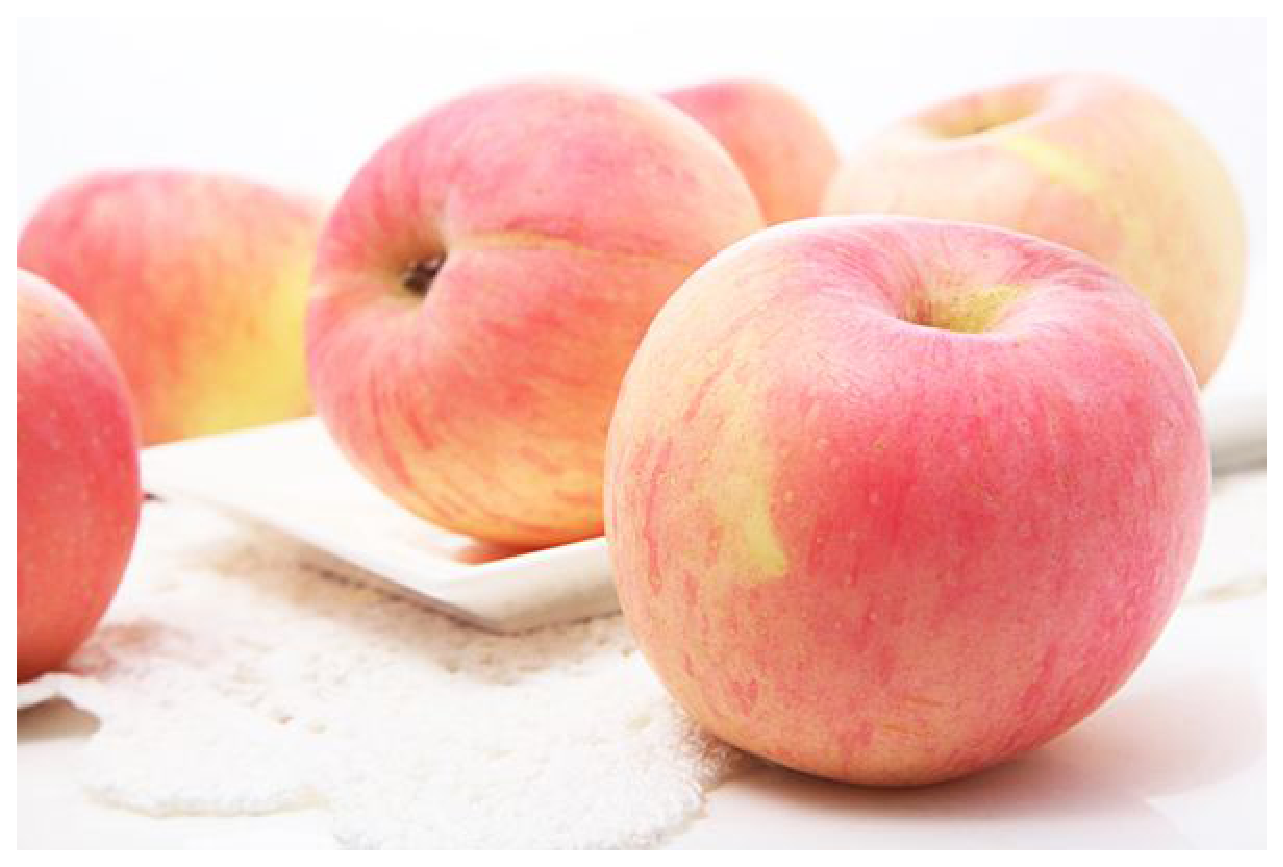
\includegraphics[scale=0.15]{apple.eps}
		\caption{apple4}
	\end{minipage}
	\caption*{apple}
	\end{figure}
	\subsection{表格}
	\begin{lstlisting}
	1、简单表格
		\begin{table}
			\caption{表格}
			\centering
			\begin{tabular}{|p{5cm} p{5cm|}}
				\hline
				1&2\\
				\hline
				\label{table1}
			\end{tabular}
		\end{table}
	\end{lstlisting}
		\begin{table}[htbp]
			\caption{表格}
			\centering
			\begin{tabular}{p{5cm} p{5cm}}
				\hline
				1&2\\
				\hline
				3&4\\
				\hline
				\label{table1}
			\end{tabular}
		\end{table}
	\begin{lstlisting}
	2、行合并
		加载支持包
		\usepackage{multirow}
		\begin{table}[h]
			\centering
			\begin{tabular}[b]{|p{2cm} |p{2cm}| p{2cm} |}
				\hline
				\multirow{2}{*}{1}&2&3\\
				\cline{2-3}
				&3&4\\
				\hline
			\end{tabular}	
		\end{table}
	\end{lstlisting}
		\begin{table}[h]
			\centering
			\begin{tabular}[b]{|p{2cm} |p{2cm}| p{2cm} |}
				\hline
				\multirow{2}{*}{1}&2&3\\
				\cline{2-3}
				&3&4\\
				\hline
			\end{tabular}		
		\end{table}
	\begin{lstlisting}
		3、列合并
			\begin{table}[h]
			\centering
			\begin{tabular}[b]{|p{2cm} |p{2cm}| p{2cm} |}
				\hline
				\multicolumn{2}{|c|}{1}&2\\
				\hline
				3&3&4\\
				\hline
			\end{tabular}		
			\end{table}	
			推荐在线表格制作:
			http://www.tablesgenerator.com/
	\end{lstlisting}
		\begin{table}[h]
		\centering
		\begin{tabular}[b]{|p{2cm} |p{2cm}| p{2cm} |}
			\hline
			\multicolumn{2}{|c|}{1}&2\\
			\hline
			3&3&4\\
			\hline
		\end{tabular}		
	\end{table}	
	\subsection{公式}
	\begin{lstlisting}
		加载数学支持包
		\usepackage{amsmath}
		1、单行公式
			\begin{equation}
				3=2+1
			\end{equation}
	\end{lstlisting}
	\begin{equation}
		3=2+1
	\end{equation}
	\begin{lstlisting}
		2、分步公式
			\begin{equation}
			\begin{split}
				a &= 3* 4 +3 \\
				&= 12+3\\
				&=15
			\end{split}
			\end{equation}
	\end{lstlisting}
		\begin{align*}
		a &= 3* 4 +3 \\
		&= 12+3\\
		&=15
	\end{align*}
	\begin{lstlisting}
		3、条件公式
			\begin{equation}
				D( x)=\begin{cases}
				1, & \text{}\\
				0 , & \text{}
				\end{cases}
			\end{equation}
	\end{lstlisting}
		\begin{equation}
		D( x)=\begin{cases}
			1, & \text{}\\
		0 , & \text{}
		\end{cases}
	\end{equation}
	\subsection{代码}
	\begin{lstlisting}
		\usepackage{listing}
		\lstset{language=python,tabsize=4} % 指定编程语言
		\begin{lstlisting}
		\ end{lstlisting}
	\end{lstlisting}
	
	\subsection{算法}
	\begin{lstlisting}
		\usepackage[ruled]{algorithm2e}
		\begin{algorithm}[H]}
		\caption{} %算法名字
		\LinesNumbered %显示行号
		\Kwln{} %输入参数
		\Kwout{} %输出
		\Repeat{}{}
		\For{}{}
		\end{algorithm }
	\end{lstlisting}
	\begin{algorithm}[H]
		\caption{算法}
		\LinesNumbered
		\KwIn{data}
		\KwOut{result}
			\Repeat{reached the stoping condition}{
			\For{$all \left ( x_{k},y_{k} \right )\epsilon D $}
			{compute the output of sample:$\hat{y}_{j}^{k}=f\left ( \beta _{j}-\theta _{j} \right ) $\;
			}
			
		}
	\end{algorithm}

	\subsection{论文引用}
	\begin{lstlisting}
		1、配置
			option=>configure texstudio=>build=>bibligraphy tool=>Biber
		2、加载支持包
			\usepackage[style=authoryear,sorting=none]{biblatex}
		3、指定引用文件
			\addbibresource{ref.bib}
		4、创建bib文件,在百度学术中复制Bib格式引用
			\parentcite{}
		5、显示引用
			\printbiblography
			
	\end{lstlisting}
	\subsection{图标转置}
	\begin{lstlisting}
		1、添加支持包
			\usepackage{rotating}
		2、 \begin{sidewaystable}
				\centering
			\end{sidewaystable}
	\end{lstlisting}
	\subsection{插入超链接}
	\begin{lstlisting}
		1、添加支持包
		   \usepackage[colorlinks,linkcolor=blue]{hyperref}
		2、\href{http://v.youku.com/}{Youku video} 
	\end{lstlisting}
	\subsection{改变字体颜色}
	\begin{lstlisting}
		\usepackage{color}
		{\color{red}}
	\end{lstlisting}
	\subsection{纸张设置}
	\begin{lstlisting}
	\documentclass[a4paper]{article}
	\usepackage[margin=1in]{geometry}
	\end{lstlisting}
	\subsection{其他}
	\begin{lstlisting}
	取消缩进 \noindent
	
	字母上下标 \mathop{min}_{}^{}
	
	添加页眉页脚
	\usepackage{fancyhdr}
	\pagestyle{fancy}
	\lhead{} 左边
	\chead{}  中间
	\rhead{} 右边
	
	字母上方箭头 \hat{}
	\end{lstlisting}
\end{document}